\documentclass[8pt,aspectratio=169]{beamer}
\usetheme{Madrid}
\usepackage{graphicx,booktabs,adjustbox,multicol,amsmath,amssymb,listings,xcolor,colortbl}
\definecolor{mlblue}{RGB}{0,102,204}
\definecolor{mlpurple}{RGB}{51,51,178}
\definecolor{mllavender}{RGB}{173,173,224}
\definecolor{mllavender2}{RGB}{193,193,232}
\definecolor{mllavender3}{RGB}{204,204,235}
\definecolor{mllavender4}{RGB}{214,214,239}
\definecolor{mlorange}{RGB}{255,127,14}
\definecolor{mlgreen}{RGB}{44,160,44}
\definecolor{mlred}{RGB}{214,39,40}
\definecolor{mlgray}{RGB}{127,127,127}
\setbeamercolor{palette primary}{bg=mllavender3,fg=mlpurple}
\setbeamercolor{palette secondary}{bg=mllavender2,fg=mlpurple}
\setbeamercolor{palette tertiary}{bg=mllavender,fg=white}
\setbeamercolor{palette quaternary}{bg=mlpurple,fg=white}
\setbeamercolor{structure}{fg=mlpurple}
\setbeamercolor{title}{fg=mlpurple}
\setbeamercolor{frametitle}{fg=mlpurple,bg=mllavender3}
\setbeamercolor{block title}{bg=mllavender2,fg=mlpurple}
\setbeamercolor{block body}{bg=mllavender4,fg=black}
\setbeamertemplate{navigation symbols}{}
\setbeamertemplate{itemize items}[circle]
\setbeamersize{text margin left=5mm,text margin right=5mm}
\newcommand{\bottomnote}[1]{\vfill\vspace{-2mm}\textcolor{mllavender2}{\rule{\textwidth}{0.4pt}}\par\vspace{1mm}{\footnotesize\textbf{\adjustbox{max width=\textwidth}{#1}}}}
\usepackage{tikz}
\usetikzlibrary{arrows.meta,positioning,shapes.geometric,calc,chains,decorations.pathmorphing,automata,fit}
\usepackage{pgfplots}
\pgfplotsset{compat=1.18}
\begin{document}

%% ============================================================
%% FRAME 1: TITLE
%% ============================================================
\begin{frame}[plain]
\vspace{1.8cm}
\begin{center}
{\Large\bfseries\color{mlpurple} Hands-On: Deploy a Token from Google Colab}\\[6mm]
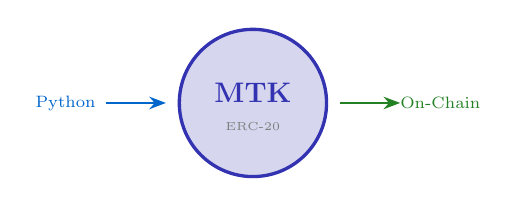
\begin{tikzpicture}[scale=0.85, every node/.style={transform shape}]
% Token icon
\draw[mlpurple, very thick, fill=mllavender4] (0,0) circle (1.1);
\node[font=\large\bfseries, mlpurple] at (0,0.15) {MTK};
\node[font=\tiny, mlgray] at (0,-0.35) {ERC-20};
% Decorative arrows
\draw[-{Stealth[length=6pt]}, mlblue, thick] (-2.2,0) -- (-1.3,0);
\draw[-{Stealth[length=6pt]}, mlgreen!80!black, thick] (1.3,0) -- (2.2,0);
\node[font=\scriptsize, mlblue] at (-2.8,0) {Python};
\node[font=\scriptsize, mlgreen!80!black] at (2.8,0) {On-Chain};
\end{tikzpicture}
\\[5mm]
{\footnotesize Prof.~Dr.~Joerg Osterrieder}\\[1mm]
{\footnotesize\color{mlgray} University Lecture Series}\\[3mm]
{\scriptsize\color{mlblue}\texttt{colab.research.google.com/github/Digital-AI-Finance/}}\\[-0.5mm]
{\scriptsize\color{mlblue}\texttt{Cryptocurrency/blob/main/notebooks/deploy\_token.ipynb}}
\end{center}
\end{frame}

%% ============================================================
%% FRAME 2: SETUP CHECKLIST
%% ============================================================
\begin{frame}{Before You Start --- Setup Checklist}
\vspace{-2mm}
\begin{columns}[T]
\begin{column}{0.55\linewidth}
\adjustbox{max width=\linewidth}{%
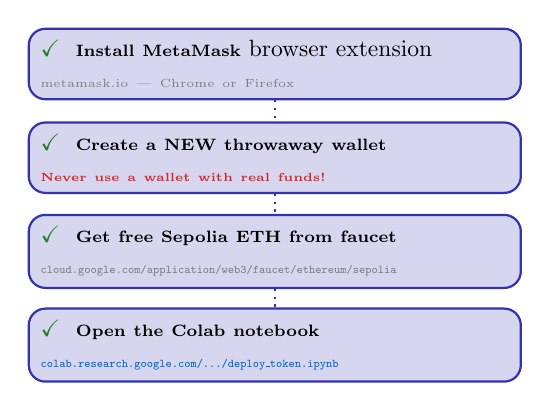
\begin{tikzpicture}[scale=0.85, every node/.style={transform shape},
  checkitem/.style={draw=mlpurple, thick, fill=mllavender4, rounded corners=6pt,
    minimum height=0.95cm, text width=7.0cm, align=left, inner sep=5pt}]

\node[checkitem] (c1) at (0,3.6) {%
  {\color{mlgreen!80!black}\bfseries$\checkmark$}~~%
  \textbf{\scriptsize Install MetaMask} browser extension\\[1pt]
  \tiny\color{mlgray} metamask.io --- Chrome or Firefox};

\node[checkitem] (c2) at (0,2.2) {%
  {\color{mlgreen!80!black}\bfseries$\checkmark$}~~%
  \textbf{\scriptsize Create a NEW throwaway wallet}\\[1pt]
  \tiny\color{mlred}\bfseries Never use a wallet with real funds!};

\node[checkitem] (c3) at (0,0.8) {%
  {\color{mlgreen!80!black}\bfseries$\checkmark$}~~%
  \textbf{\scriptsize Get free Sepolia ETH from faucet}\\[1pt]
  \tiny\color{mlgray}\texttt{cloud.google.com/application/web3/faucet/ethereum/sepolia}};

\node[checkitem] (c4) at (0,-0.6) {%
  {\color{mlgreen!80!black}\bfseries$\checkmark$}~~%
  \textbf{\scriptsize Open the Colab notebook}\\[1pt]
  \tiny\color{mlblue}\texttt{colab.research.google.com/.../deploy\_token.ipynb}};

% Connecting line
\draw[mlpurple, thick, dotted] (c1.south) -- (c2.north);
\draw[mlpurple, thick, dotted] (c2.south) -- (c3.north);
\draw[mlpurple, thick, dotted] (c3.south) -- (c4.north);

\end{tikzpicture}%
}%
\end{column}
\begin{column}{0.43\linewidth}
\adjustbox{max width=\linewidth}{%
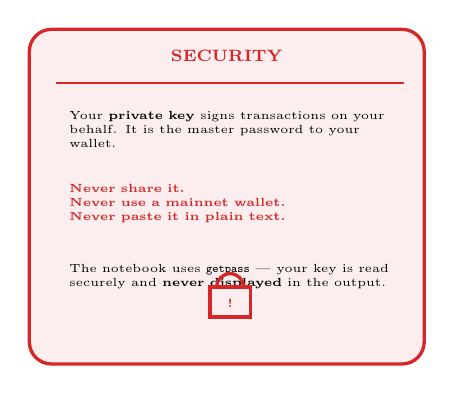
\begin{tikzpicture}[scale=0.85, every node/.style={transform shape}]
% Warning box
\draw[mlred, very thick, fill=mlred!8, rounded corners=8pt] (-0.1,-0.8) rectangle (5.8,4.2);
\node[font=\scriptsize\bfseries, mlred] at (2.85,3.8) {SECURITY};

\draw[mlred, thick] (0.3,3.4) -- (5.5,3.4);

\node[font=\tiny, text width=4.8cm, align=left] at (2.9,2.7) {%
  Your \textbf{private key} signs transactions on your behalf. It is the master password to your wallet.};

\node[font=\tiny, text width=4.8cm, align=left] at (2.9,1.6) {%
  \textbf{\color{mlred}Never share it.}\\
  \textbf{\color{mlred}Never use a mainnet wallet.}\\
  \textbf{\color{mlred}Never paste it in plain text.}};

\node[font=\tiny, text width=4.8cm, align=left] at (2.9,0.5) {%
  The notebook uses \texttt{getpass} --- your key is read securely and \textbf{never displayed} in the output.};

% Lock icon
\draw[mlred, very thick] (2.6,-0.1) rectangle (3.2,0.35);
\draw[mlred, very thick] (2.7,0.35) arc (180:0:0.2) -- (3.1,0.35);
\node[font=\tiny\bfseries, mlred] at (2.9,0.1) {!};

\end{tikzpicture}%
}%
\end{column}
\end{columns}

\bottomnote{All tools are free. Sepolia ETH is test money with no real value --- perfect for learning.}
\end{frame}

%% ============================================================
%% FRAME 3: UNDERSTANDING THE CONTRACT CODE
%% ============================================================
\begin{frame}{Understanding the Contract Code}
\vspace{-2mm}
\begin{columns}[T]
\begin{column}{0.48\linewidth}
\adjustbox{max width=\linewidth}{%
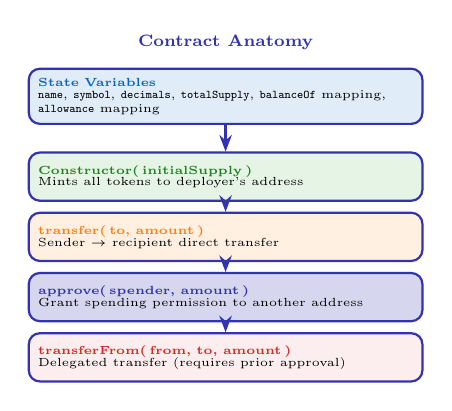
\begin{tikzpicture}[scale=0.85, every node/.style={transform shape},
  partbox/.style={draw=mlpurple, thick, rounded corners=4pt,
    minimum height=0.72cm, text width=5.6cm, align=left, inner sep=4pt, font=\tiny}]

\node[font=\scriptsize\bfseries, mlpurple] at (2.9,5.0) {Contract Anatomy};

\node[partbox, fill=mlblue!12] (p1) at (2.9,4.2) {%
  \textbf{\color{mlblue}State Variables}\\[-1pt]
  \texttt{name}, \texttt{symbol}, \texttt{decimals}, \texttt{totalSupply},
  \texttt{balanceOf} mapping, \texttt{allowance} mapping};

\node[partbox, fill=mlgreen!12] (p2) at (2.9,3.0) {%
  \textbf{\color{mlgreen!80!black}Constructor(\,initialSupply\,)}\\[-1pt]
  Mints all tokens to deployer's address};

\node[partbox, fill=mlorange!12] (p3) at (2.9,2.1) {%
  \textbf{\color{mlorange}transfer(\,to, amount\,)}\\[-1pt]
  Sender $\rightarrow$ recipient direct transfer};

\node[partbox, fill=mllavender4] (p4) at (2.9,1.2) {%
  \textbf{\color{mlpurple}approve(\,spender, amount\,)}\\[-1pt]
  Grant spending permission to another address};

\node[partbox, fill=mlred!8] (p5) at (2.9,0.3) {%
  \textbf{\color{mlred}transferFrom(\,from, to, amount\,)}\\[-1pt]
  Delegated transfer (requires prior approval)};

% Connecting arrows
\draw[-{Stealth[length=6pt]}, mlpurple, thick] (p1.south) -- (p2.north);
\draw[-{Stealth[length=6pt]}, mlpurple, thick] (p2.south) -- (p3.north);
\draw[-{Stealth[length=6pt]}, mlpurple, thick] (p3.south) -- (p4.north);
\draw[-{Stealth[length=6pt]}, mlpurple, thick] (p4.south) -- (p5.north);

\end{tikzpicture}%
}%
\end{column}
\begin{column}{0.50\linewidth}
\vspace{1mm}
{\scriptsize\bfseries\color{mlblue} Why self-contained?}\\[1pt]
{\tiny No npm, no OpenZeppelin imports. The contract is defined
inline so \texttt{py-solc-x} can compile it directly in Colab
without any external dependencies.}\\[4mm]

{\scriptsize\bfseries\color{mlgreen!80!black} Why 18 decimals?}\\[1pt]
{\tiny Matches ETH precision. Solidity has no floating point,
so 1 token = $10^{18}$ base units. When you deploy with
\texttt{initialSupply = 500{,}000}, the contract stores
$500{,}000 \times 10^{18}$ internally.}\\[4mm]

{\scriptsize\bfseries\color{mlorange} Why a constructor argument?}\\[1pt]
{\tiny You choose the total supply at deploy time. The constructor
runs exactly once when the contract is created, minting all
tokens to your address (the deployer).}\\[4mm]

{\scriptsize\bfseries\color{mlpurple} ERC-20 standard}\\[1pt]
{\tiny These five elements (\texttt{balanceOf}, \texttt{transfer},
\texttt{approve}, \texttt{allowance}, \texttt{transferFrom}) are
the minimal ERC-20 interface. Any wallet or DEX that speaks
ERC-20 can interact with your token.}
\end{column}
\end{columns}

\bottomnote{The contract is ~40 lines of Solidity --- fully self-contained, no imports needed, compiles in Python.}
\end{frame}

%% ============================================================
%% FRAME 4: LIVE CODING WALKTHROUGH
%% ============================================================
\begin{frame}{Live Coding Walkthrough --- What Each Cell Does}
\vspace{-2mm}
\begin{center}
\adjustbox{max width=\textwidth, max totalheight=6.5cm}{%
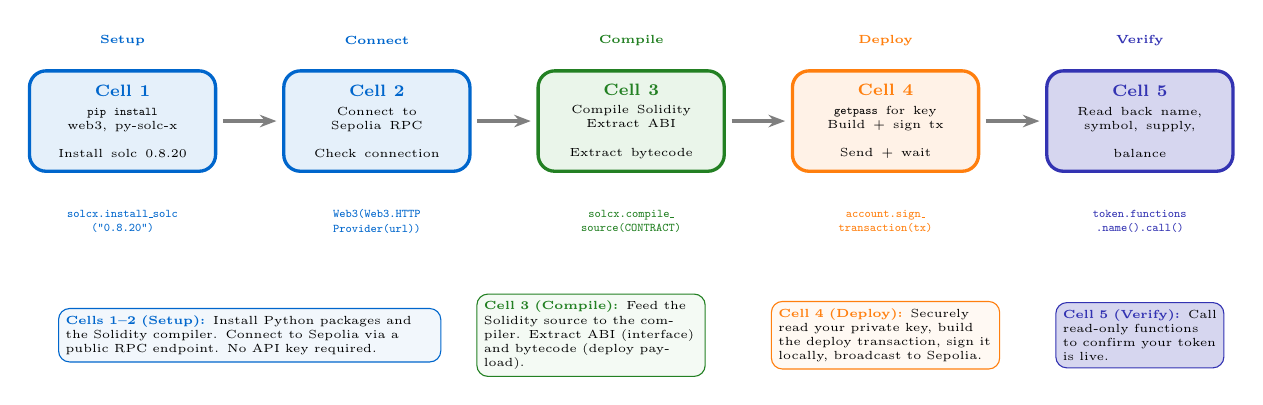
\begin{tikzpicture}[scale=0.85, every node/.style={transform shape}]

% --- Cell 1: Install ---
\node[draw=mlblue, very thick, fill=mlblue!10, rounded corners=6pt,
  minimum height=1.5cm, text width=2.5cm, align=center, inner sep=4pt]
  (c1) at (0,1.5) {%
  \textbf{\scriptsize\color{mlblue} Cell 1}\\[2pt]
  \tiny\texttt{pip install}\\
  \tiny web3, py-solc-x\\
  \tiny Install solc 0.8.20};
\node[font=\tiny, mlblue, text width=2.6cm, align=center] at (0,-0.0) {%
  \texttt{solcx.install\_solc}\\
  \texttt{("0.8.20")}};
\node[font=\tiny\bfseries, mlblue] at (0,2.7) {Setup};

% Arrow 1->2
\draw[-{Stealth[length=6pt]}, mlgray, very thick] (1.5,1.5) -- (2.3,1.5);

% --- Cell 2: Connect ---
\node[draw=mlblue, very thick, fill=mlblue!10, rounded corners=6pt,
  minimum height=1.5cm, text width=2.5cm, align=center, inner sep=4pt]
  (c2) at (3.8,1.5) {%
  \textbf{\scriptsize\color{mlblue} Cell 2}\\[2pt]
  \tiny Connect to\\
  \tiny Sepolia RPC\\
  \tiny Check connection};
\node[font=\tiny, mlblue, text width=2.6cm, align=center] at (3.8,-0.0) {%
  \texttt{Web3(Web3.HTTP}\\
  \texttt{Provider(url))}};
\node[font=\tiny\bfseries, mlblue] at (3.8,2.7) {Connect};

% Arrow 2->3
\draw[-{Stealth[length=6pt]}, mlgray, very thick] (5.3,1.5) -- (6.1,1.5);

% --- Cell 3: Compile ---
\node[draw=mlgreen!80!black, very thick, fill=mlgreen!10, rounded corners=6pt,
  minimum height=1.5cm, text width=2.5cm, align=center, inner sep=4pt]
  (c3) at (7.6,1.5) {%
  \textbf{\scriptsize\color{mlgreen!80!black} Cell 3}\\[2pt]
  \tiny Compile Solidity\\
  \tiny Extract ABI\\
  \tiny Extract bytecode};
\node[font=\tiny, mlgreen!80!black, text width=2.6cm, align=center] at (7.6,-0.0) {%
  \texttt{solcx.compile\_}\\
  \texttt{source(CONTRACT)}};
\node[font=\tiny\bfseries, mlgreen!80!black] at (7.6,2.7) {Compile};

% Arrow 3->4
\draw[-{Stealth[length=6pt]}, mlgray, very thick] (9.1,1.5) -- (9.9,1.5);

% --- Cell 4: Deploy ---
\node[draw=mlorange, very thick, fill=mlorange!10, rounded corners=6pt,
  minimum height=1.5cm, text width=2.5cm, align=center, inner sep=4pt]
  (c4) at (11.4,1.5) {%
  \textbf{\scriptsize\color{mlorange} Cell 4}\\[2pt]
  \tiny \texttt{getpass} for key\\
  \tiny Build + sign tx\\
  \tiny Send + wait};
\node[font=\tiny, mlorange, text width=2.6cm, align=center] at (11.4,-0.0) {%
  \texttt{account.sign\_}\\
  \texttt{transaction(tx)}};
\node[font=\tiny\bfseries, mlorange] at (11.4,2.7) {Deploy};

% Arrow 4->5
\draw[-{Stealth[length=6pt]}, mlgray, very thick] (12.9,1.5) -- (13.7,1.5);

% --- Cell 5: Verify ---
\node[draw=mlpurple, very thick, fill=mllavender4, rounded corners=6pt,
  minimum height=1.5cm, text width=2.5cm, align=center, inner sep=4pt]
  (c5) at (15.2,1.5) {%
  \textbf{\scriptsize\color{mlpurple} Cell 5}\\[2pt]
  \tiny Read back name,\\
  \tiny symbol, supply,\\
  \tiny balance};
\node[font=\tiny, mlpurple, text width=2.6cm, align=center] at (15.2,-0.0) {%
  \texttt{token.functions}\\
  \texttt{.name().call()}};
\node[font=\tiny\bfseries, mlpurple] at (15.2,2.7) {Verify};

% --- Bottom explanation boxes ---
\node[draw=mlblue, fill=mlblue!5, rounded corners=4pt, font=\tiny,
      inner sep=3pt, text width=5.5cm, align=left]
      at (1.9,-1.7) {%
      \textbf{\color{mlblue}Cells 1--2 (Setup):} Install Python packages
      and the Solidity compiler. Connect to Sepolia
      via a public RPC endpoint. No API key required.};

\node[draw=mlgreen!80!black, fill=mlgreen!5, rounded corners=4pt, font=\tiny,
      inner sep=3pt, text width=3.2cm, align=left]
      at (7.0,-1.7) {%
      \textbf{\color{mlgreen!80!black}Cell 3 (Compile):}
      Feed the Solidity source to the compiler.
      Extract ABI (interface) and bytecode (deploy payload).};

\node[draw=mlorange, fill=mlorange!5, rounded corners=4pt, font=\tiny,
      inner sep=3pt, text width=3.2cm, align=left]
      at (11.4,-1.7) {%
      \textbf{\color{mlorange}Cell 4 (Deploy):}
      Securely read your private key, build the deploy
      transaction, sign it locally, broadcast to Sepolia.};

\node[draw=mlpurple, fill=mllavender4, rounded corners=4pt, font=\tiny,
      inner sep=3pt, text width=2.3cm, align=left]
      at (15.2,-1.7) {%
      \textbf{\color{mlpurple}Cell 5 (Verify):}
      Call read-only functions to confirm your token is live.};

\end{tikzpicture}%
}%
\end{center}

\bottomnote{Five cells, five minutes. Each cell builds on the previous one --- run them top to bottom in order.}
\end{frame}

%% ============================================================
%% FRAME 5: AFTER YOU DEPLOY
%% ============================================================
\begin{frame}{After You Deploy --- What to Do Next}
\vspace{-2mm}
\begin{columns}[T]
\begin{column}{0.52\linewidth}
\adjustbox{max width=\linewidth}{%
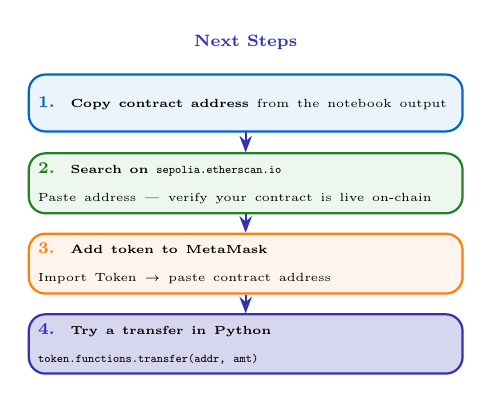
\begin{tikzpicture}[scale=0.85, every node/.style={transform shape},
  stepbox/.style={draw=mlpurple, thick, fill=mllavender4, rounded corners=6pt,
    minimum height=0.85cm, text width=6.2cm, align=left, inner sep=4pt}]

\node[font=\scriptsize\bfseries, mlpurple] at (3.2,4.8) {Next Steps};

\node[stepbox, draw=mlblue, fill=mlblue!8] (s1) at (3.2,3.9) {%
  {\scriptsize\bfseries\color{mlblue} 1.}~~%
  {\tiny\bfseries Copy contract address} {\tiny from the notebook output}};

\node[stepbox, draw=mlgreen!80!black, fill=mlgreen!8] (s2) at (3.2,2.7) {%
  {\scriptsize\bfseries\color{mlgreen!80!black} 2.}~~%
  {\tiny\bfseries Search on \texttt{sepolia.etherscan.io}}\\
  {\tiny Paste address --- verify your contract is live on-chain}};

\node[stepbox, draw=mlorange, fill=mlorange!8] (s3) at (3.2,1.5) {%
  {\scriptsize\bfseries\color{mlorange} 3.}~~%
  {\tiny\bfseries Add token to MetaMask}\\
  {\tiny Import Token $\rightarrow$ paste contract address}};

\node[stepbox, draw=mlpurple, fill=mllavender4] (s4) at (3.2,0.3) {%
  {\scriptsize\bfseries\color{mlpurple} 4.}~~%
  {\tiny\bfseries Try a transfer in Python}\\
  {\tiny\texttt{token.functions.transfer(addr, amt)}}};

% Connecting arrows
\draw[-{Stealth[length=6pt]}, mlpurple, thick] (s1.south) -- (s2.north);
\draw[-{Stealth[length=6pt]}, mlpurple, thick] (s2.south) -- (s3.north);
\draw[-{Stealth[length=6pt]}, mlpurple, thick] (s3.south) -- (s4.north);

\end{tikzpicture}%
}%
\end{column}
\begin{column}{0.46\linewidth}
\adjustbox{max width=\linewidth}{%
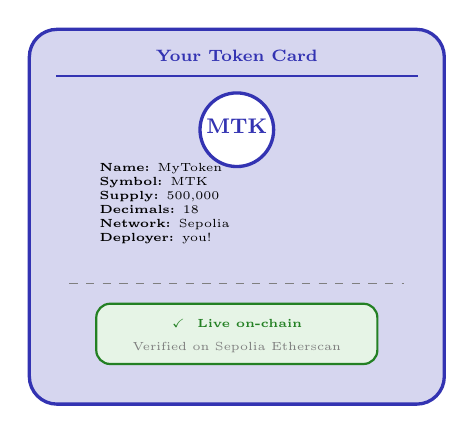
\begin{tikzpicture}[scale=0.85, every node/.style={transform shape}]
% Card background
\draw[mlpurple, very thick, fill=mllavender4, rounded corners=10pt]
  (-0.2,-0.6) rectangle (6.0,5.0);

% Title
\node[font=\scriptsize\bfseries, mlpurple] at (2.9,4.6) {Your Token Card};
\draw[mlpurple, thick] (0.2,4.3) -- (5.6,4.3);

% Token circle
\draw[mlpurple, very thick, fill=white] (2.9,3.5) circle (0.55);
\node[font=\small\bfseries, mlpurple] at (2.9,3.55) {MTK};

% Details
\node[font=\tiny, text width=4.5cm, align=left] at (3.1,2.4) {%
  \textbf{Name:} MyToken\\
  \textbf{Symbol:} MTK\\
  \textbf{Supply:} 500,000\\
  \textbf{Decimals:} 18\\
  \textbf{Network:} Sepolia\\
  \textbf{Deployer:} you!};

% Divider
\draw[mlgray, thin, dashed] (0.4,1.2) -- (5.4,1.2);

% Badge
\draw[mlgreen!80!black, thick, fill=mlgreen!12, rounded corners=5pt]
  (0.8,0.0) rectangle (5.0,0.9);
\node[font=\tiny\bfseries, mlgreen!80!black] at (2.9,0.6) {$\checkmark$~~Live on-chain};
\node[font=\tiny, mlgray] at (2.9,0.25) {Verified on Sepolia Etherscan};

\end{tikzpicture}%
}%
\end{column}
\end{columns}

\bottomnote{Colab notebook: \texttt{colab.research.google.com/github/Digital-AI-Finance/Cryptocurrency/blob/main/notebooks/deploy\_token.ipynb}}
\end{frame}

\end{document}
